\section[Mitochondrial phylogenetic reconstruction]{Mitochondrial phylogenetic reconstruction - the power house of the phylogenies}
\label{cascade-sec:mitochondria}

While phylogenetic reconstruction is a well-established method for genetic variants from canonical chromosomes to study metastatic progression and timing of evolutionary divergence \cite{Deshwar2015,Brown2017,Hu2019}, there are multiple issues. In \autoref{variantcalling-sec:phylo} and \autoref{variantcalling-sec:clonal}, we showed how important the proper variant calling method is to \remove{accurately} recover phylogenies and clonal patterns\add{ accurately}. In addition, using somatic variants to reconstruct phylogenies is a flawed concept to begin with. 

Most models studying genetic variation assume neutral evolution of the DNA loci \cite{Kimura1968,Lynch1989}, but cancers almost exclusively exhibit positive selection \cite{Cannataro2018}. \change{And}{Moreover,} while passenger mutations might not directly affect \add{the} \change{fitness of the cell}{cell's fitness}, they only exist due to the link to the driver mutation and \remove{therefore} provide little to no additional information gain in addition to the driver. Furthermore, while in small populations, genetic drift as a stochastic process overpowers selective processes (fitness coefficient $s$) and can therefore be assumed to be neutral, in larger populations $N_e$ (effective population size) where \autoref{mmf-eq:neutralSelection} does not hold true, mutations are under selective pressure \cite{EyreWalker2007}.
\begin{equation}
N_e \cdot s \ll 1 \label{mmf-eq:neutralSelection}
\end{equation}
\myequation[\ref{mmf-eq:neutralSelection}]{Selective pressure with effective population size}
%we need to squish this a bit otherwise it looks weird
\vspace{-3em}
In summary, we can assume that with cancer cell growth, positive selection through treatment, and tumour-microenvironmental niches, almost all assumptions of the coalescent theory \cite{Kingman1982} are not applicable for tumour samples and therefore, methods using somatic variants and their respective results need to be selected and evaluated carefully.

To tackle this issue and assist with \change{the interpretation of}{interpreting} phylogenetic reconstruction results, we adjusted a method used in single-cell sequencing to track clonal expansion with mitochondrial somatic mutations \cite{Ludwig2019} to be usable \change{for}{with} standard bulk sequencing. Mitochondrial variants are an ideal source of clonality information because the mutation rate is significantly higher than nuclear DNA due to the missing proofreading and repair mechanisms, \change{which allows}{allowing} very granular separation in a shorter time\remove{ period}. Additionally, while \remove{there are several diseases caused by} defects in mitochondria\add{ cause several diseases}, such as Kearns-Sayre syndrome \cite{Harvey1992}, MERRF \cite{Adam1993} and MELAS \cite{Hirano1992}, they usually follow a mendelian inheritance pattern and are hereditary and not somatically acquired. In the cancer context, somatic mutations in mitochondrial DNA are assumed to be approximately neutral, with a possible selection pressure towards healthy ageing and negative selection in cancer \cite{Rodell2013,Yuan2020}.

\subsection{Method}
\label{cascade-sec:mitoMethod}

First, a pileup of all mitochondrial positions was performed. Before, the pileup we preselected reads which uniquely mapped to the mitochondrial genome and only retained high mapping-quality reads. Then the nucleotide counts in each position were transformed into a MultiEssayExperiment \cite{Ramos2017} for final analysis in R. The preprocessing code can be found in \autoref{lst-cascadeAppendix:mitoPreProcessing}.

The final MultiEssayExperiment was then read into R, and quality metrics \add{were }applied to exclude samples with \change{not enough}{insufficient} coverage on the mitochondrial contig. Our analysed WGS samples showed an extensive coverage of mitochondrial DNA\change{, however}{. However}, WES library preparation procedures might restrict coverage through hybridisation pulldown. Patient CA-I had \remove{a coverage of} more than 100x \add{coverage }for all but the germline sample, which only had an overall coverage of 17x. Similarly, patient CA-L showed lower depth for the germline sample (127x) but a generally high coverage for all tumour samples (mean: 543x, min: 138x). All other Patients (CA-A/J/K) where samples were sequenced with WGS exhibited a coverage of more than 200x, even for low-performing samples with a median depth of \num{67916}, \num{45603}, and \num{49726} per sample~(\autoref{fig:mtCoverage}).

\begin{figure}[hbt]
\centering
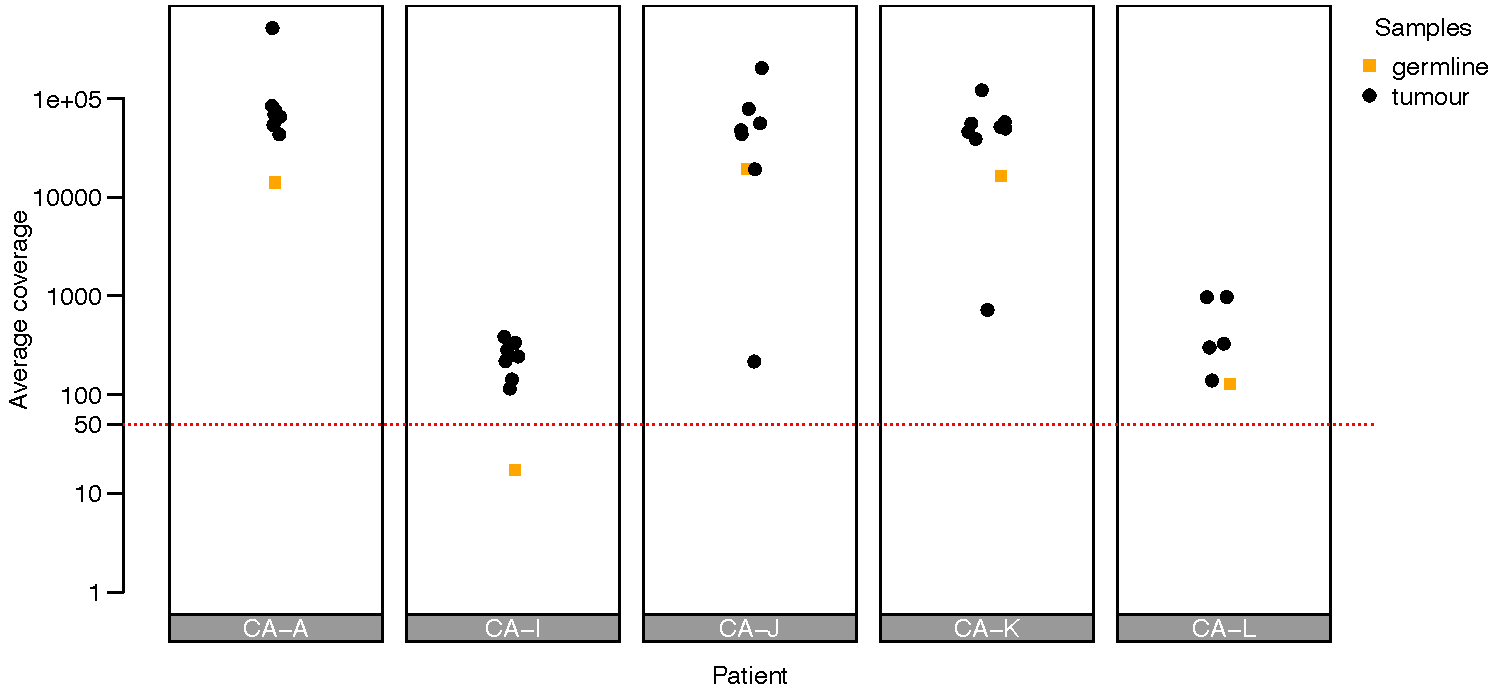
\includegraphics[width=.99\linewidth]{Figures/CASCADE/mito/mtCoverage}
\vspace{-1em}
\caption[Average coverage of mitochondrial DNA of CASCADE patients]{Average coverage of mitochondrial DNA of CASCADE patients: Orange squares show germline sample for each patient; black points show tumour samples; horizontal red dotted line shows quality cut off suggested by \protect\textcite{Ludwig2019}} \label{fig:mtCoverage}
\end{figure}


Th\change{is}{ese metrics} proved that even without specifically enriching for mitochondrial DNA, most samples \remove{will }contained enough tumour reads for this analysis.

To ensure optimal results, we excluded all samples with an average coverage of less than 50x. This exclusion meant we removed the germline sample for patient CA-I\change{, h}{. H}owever, as we expected the germline sample to be the ancestral state for all samples, this has virtually no effect on the reconstruction procedure. Additionally, we were more interested in the relationships between the tumour sample, which was still accessible even with the removed germline sample.

In contrast to the simple Hamming distance used for the presence-absence vector representation of canonical somatic variants (\autoref{cascade-sec:phylo}), for mitochondrial variants, we employed an allele frequency ($vaf$) based distance (\autoref{eq:mitoDist}) of two samples~$s_i$ and $s_j$. The difference in read support was normalised with the product of the total allelic depth~$cov$ and summed up at all sites of variation~$v$.

\begin{equation}
mitoDist(s_i,s_j) = \sum_{v \in Variants} \left| \frac{vaf_{s_i}(v) \cdot cov_{s_i}(v) - vaf_{s_j}(v) \cdot cov_{s_j}(v)}{cov_{s_i}(v) \cdot cov_{s_j}(v)} \right| \label{eq:mitoDist}
\end{equation}
\myequation[\ref{eq:mitoDist}]{Mitochondrial variants based distance function of two samples}

This distance was only calculated for variant sites where both samples had at least a coverage of 100x to have a representative sampling of the allelic prevalence in each sample, as a human cell usually has more than 100 mitochondria \cite{Cole2016}.


\subsection{Results}
\label{cascade-sec:mitoResults}
While the mitochondrial variants analysis only used a fraction of the size of the genomic DNA loci and therefore most likely violates the infinite sites assumption \cite{Kimura1969}, it was still able to generate an orthogonal view of the heterogeneity and trajectory of the multi-regional samples in each patient.

\subsubsection{Patient CA-A}

While the separation of progression (11, 47, 55, and 59) and stable (26, 31, 41, and 57) disease sites was already visible in the somatic phylogeny, the bottleneck of treatment and new metastasis is more \change{obvious}{evident} in the mitochondrial phylogeny. However, the individual resolution of splits appeared to be lower for the mitochondrial reconstruction, as seen in \autoref{fig:CA99mitoPhylo}.


\begin{figure}[h]
\centering
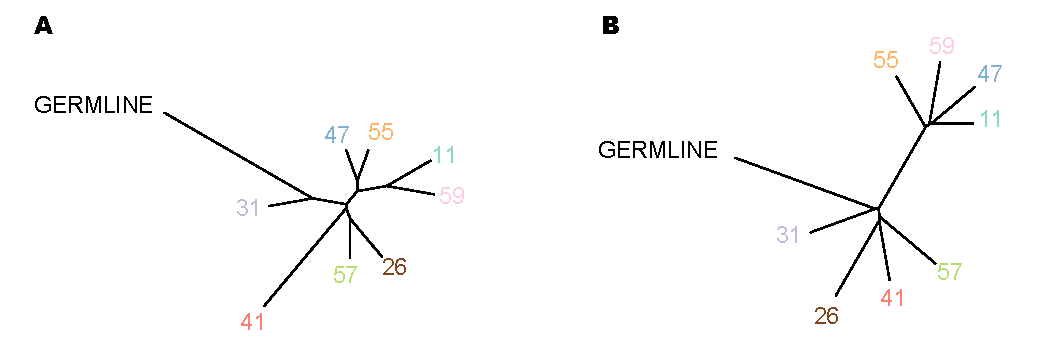
\includegraphics[width=.99\linewidth]{Figures/CASCADE/mito/CA99SomVsMitoPhylo.pdf}
\caption[Mitochondrial and somatic phylogenetic reconstruction of CA-A]{Mitochondrial and somatic phylogenetic reconstruction of CA-A: Somatic variants based reconstruction (A) and mitochondrial variants based reconstruction (B)} \label{fig:CA99mitoPhylo}
\end{figure}

\subsubsection{Patient CA-I}

Neither the somatic \remove{variants} nor the mitochondrial variants resolved the evolutionary trajectory in a granular fashion. The slightly longer stem of shared variants in the mitochondrial phylogeny was most likely due to the low coverage of the germline sample. Similar to all other patients, the substructure of the samples was changed. While \remove{using} the somatic variants showed sample 566 as the closest to the germline sample, the mitochondrial variant phylogeny instead indicated sample 559 as the closest (\Autoref{fig:mtCoverage,fig:CA51mitoPhylo}).


\begin{figure}[ht]
\centering
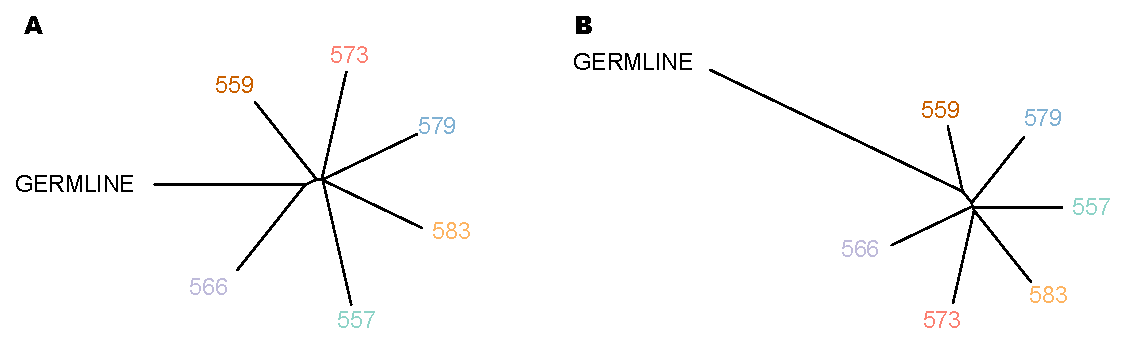
\includegraphics[width=.99\linewidth]{Figures/CASCADE/mito/CA51SomVsMitoPhylo.pdf}
\caption[Mitochondrial and somatic phylogenetic reconstruction of CA-I]{Mitochondrial and somatic phylogenetic reconstruction of CA-I: Somatic variants based reconstruction (A) and mitochondrial variants based reconstruction (B)} \label{fig:CA51mitoPhylo}
\end{figure}


\subsubsection{Patient CA-J}

The mitochondrial reconstruction presented sample 2 as a member of the more genetically complex samples 20, 24, 32, and 42 \change{in spite of}{despite} the missing \textit{TP53} mutation. Sample 28, on the other hand, \remove{which }showed almost no evolutionary distance to the normal sample in the somatic analysis, \add{but} presented as a substantial outlier\add{ in the mitochondrial data}. This disconnect showed that the TP53 mutations of samples 20, 24, 32, and 42 \change{was}{were} likely acquired after the seeding of the distant sites like sample 2 in the adrenal gland. The difference in distance to the normal sample for sample 28 was likely due to a ``cold`` primary site of disease with little cell proliferation, which\remove{, however,} still accumulated mitochondrial mutations \cite{Abascal2021} (\autoref{tab:ca80cnv}, \autoref{fig:CA80mitoPhylo}).

\begin{figure}[ht]
\centering
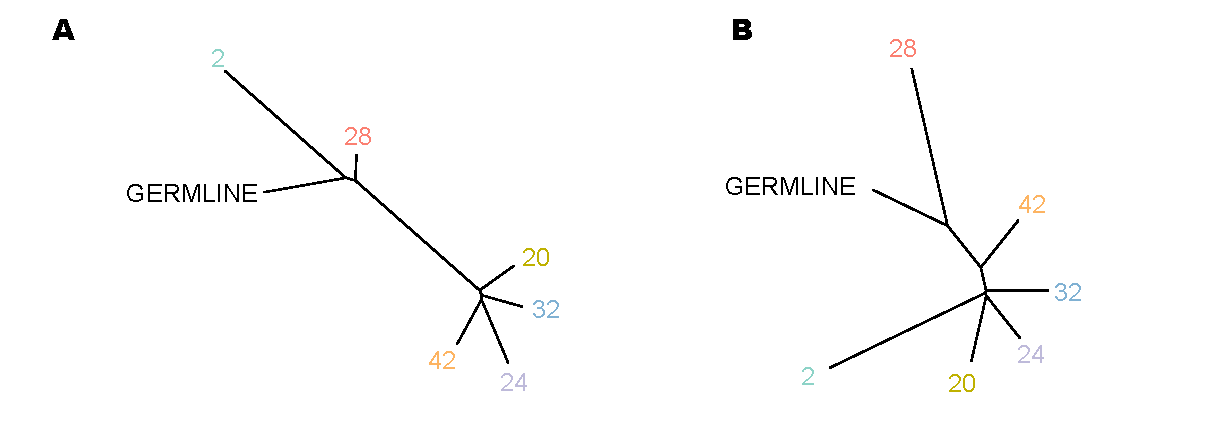
\includegraphics[width=.99\linewidth]{Figures/CASCADE/mito/CA80SomVsMitoPhylo.pdf}
\caption[Mitochondrial and somatic phylogenetic reconstruction of CA-J]{Mitochondrial and somatic phylogenetic reconstruction of CA-J: Somatic variants based reconstruction (A) and mitochondrial variants based reconstruction (B)} \label{fig:CA80mitoPhylo}
\end{figure}


\subsubsection{Patient CA-K}

In contrast to the somatic variant phylogeny, which showed an outgroup of samples 8 and 9, with a second cluster of samples 4, 5, and 6, the mitochondrial data supported a different  split into two groups. These groups almost perfectly bifurcated the samples into those derived from the left and right sided disease sites, with sample 6 being the only sample from  the right side clustered with the left lung and brain samples 8, 9, and 13. These data suggested that while only samples 8 and 9 showed a whole genome duplication and the \textit{APC} ``stop gained`` mutation, they were more closely related to the other samples than assumed from the somatic variant analysis and probably were seeded by the same cells (\autoref{tab:ca82cnv}, \Autoref{fig:ca82heatmap,fig:CA82mitoPhylo}).

\begin{figure}[ht]
\centering
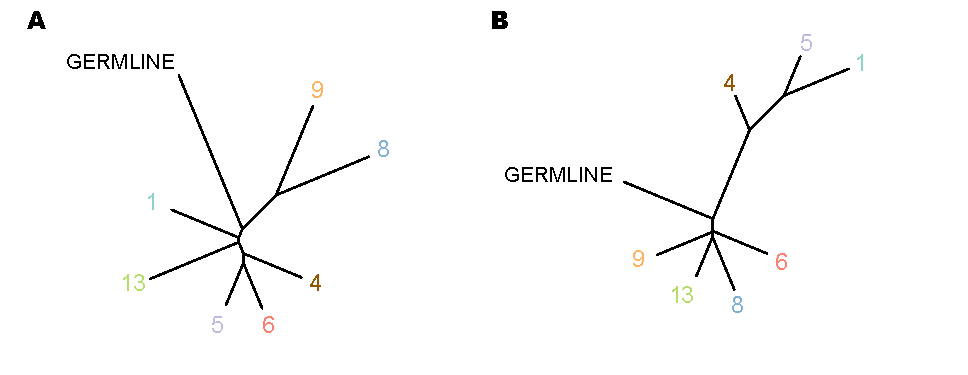
\includegraphics[width=.99\linewidth]{Figures/CASCADE/mito/CA82SomVsMitoPhylo.pdf}
\caption[Mitochondrial and somatic phylogenetic reconstruction of CA-K]{Mitochondrial and somatic phylogenetic reconstruction of CA-K: Somatic variants based reconstruction (A) and mitochondrial variants based reconstruction (B)} \label{fig:CA82mitoPhylo}
\end{figure}


\subsubsection{Patient CA-L}
While the somatic variants linked the small cell carcinoma samples P.1 and 8 together, the mitochondrial analysis showed that the closest relative to P.1 was P.2. As both of the progression samples were taken 14 months ahead of the death of the patient, this agreed with the clinical history of the samples better. Additionally, instead of grouping the\remove{ the} adenocarcinoma samples 17A and 26\remove{ together}, the mitochondrial phylogeny suggested that while they share a common resistance mechanism (EGFR~T790M), it might have been acquired in parallel instead of being seeded from the same lesion, as all samples other than the P.1/2 samples were not grouped\remove{ together}. Lastly, the closeness of sample 8 and the germline sample possibly indicated the presence of small cell disease already ``before`` the progression samples were collected. However, the FFPE conservation of the P samples could have altered the molecular clock and influenced the branching site on the tree (\Autoref{fig:ca86heatmap,fig:CA86mitoPhylo}).

\begin{figure}[ht]
\centering
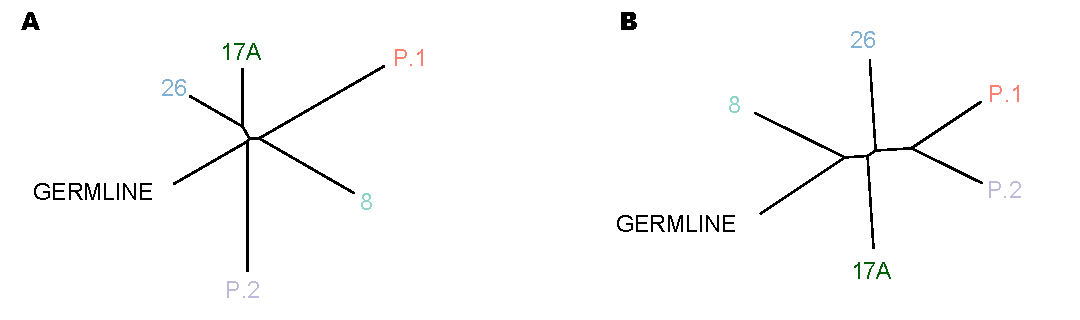
\includegraphics[width=.99\linewidth]{Figures/CASCADE/mito/CA86SomVsMitoPhylo.pdf}
\caption[Mitochondrial and somatic phylogenetic reconstruction of CA-L]{Mitochondrial and somatic phylogenetic reconstruction of CA-L: Somatic variants based reconstruction (A) and mitochondrial variants based reconstruction (B)} \label{fig:CA86mitoPhylo}
\end{figure}

\subsection{Summary}
With the analysis of the mitochondrial history of samples, we could shed some light on the timing of lesions and the development of resistance mechanisms, which is not heavily influenced by the treatment and its selection pressure. While the infinite sites hypothesis does not hold true for mitochondrial DNA, due to the limited sites and reduced repair mechanisms, the selection pressure of treatment and their resistance mechanisms parallel evolution bias in the analysis of multiple related tumour samples also violates multiple assumptions for phylogenetic reconstruction when using somatic variants. 

\note{massive rewrite}Neither options come without pitfalls and caveats, but this method could offer an alternate view on the history and seeding time of lesions and their kinship using data that was previously discarded but was abundantly available. This approach is also available at virtually no additional cost, as mitochondrial variants can be readily detected from standard WGS and WES. As mitochondrial DNA analysis has recently been moved into the spotlight as a biomarker for stress and mortality \cite{Trumpff2021} and other diseases \cite{Cushen2022}, we were interested similar to see if tissue mitochondrial DNA analysis, like circulating mitochondrial DNA, could unlock another multi-omics dimension. Furthermore, mitochondrial DNA was successfully used to distinguish clones in single-cell sequencing \cite{Ludwig2019}. 

While certain aspects of evolutionary trajectory and patterns are conserved between the nuclear DNA and the mitochondrial DNA, many are not. These differences might be caused by the reduced granularity of the mitochondrial analysis, where the median number of somatic variants was 345 (min: 128, max 5401) over the median of 23252 (min: 10947, max: 64580) in the nuclear DNA, however they could also be caused by a different biological process. The method is not an alternative to nuclear DNA phylogeny, but rather points out a need for further investigation. The reconstruction methods should be approximately equivalent with the current biological insight. However, the discrepancy of results from nuclear and mitochondrial DNA phylogenetic reconstruction, warrants further investigation of mitochondrial evolution in the cancer setting, outside the scope of this work.